\chapter{Solution}
This Chapter will explain the details of the implementation, and our methodology. We dive into each component for a thorough explanation, and RTL sketches for each.


\section{Methodology}
As this exercise is to improve the single-cycle version of the MIPS-processor. It was natural to use the design from Exercise 1 \cite{ex1report} as a starting point.
The new components needed to realize a pipelined designed were sketched out on paper. We used a bottom up approach, designing the new modules first, and integrated them to the system as they completed.

\section{Implementation}
Figure \ref{toplevel} shows all major components in the system. 
The Data memory and Instruction memory was provided in the exercise.
The components that were implemented in Exercise 1, and improved to support multi-cycle operation is as follows:

\begin{description}
  \item[Control] \hfill \\
  The control unit takes the opcode of an instruction, and sets the appropriate control signals. The statefulness that was needed in the single-cycle version has been removed, and the unit is now stateless.  
  \item[Program counter (PC)] \hfill \\
  The program counter keeps track off the address to the next instruction to be executed. If there is a branch, the PC will receive the branch address from the Branch unit. The PC may stall, if there is a control hazard.
  \item[ALU] \hfill \\
  The heart of the processor, the ALU performs an operation issued by the control unit and outputs a result along with a zero signal. This module has been updated to support forwarded data.
  \item[Registers] \hfill \\
  The register bank is the short term memory of the architecture, feeding operands to the ALU, and receiving data which may be stored based on control signals.
\end{description}

To make the processor pipelined, we need to introduce a number of new modules.

\begin{description}
  \item[Branch] \hfill \\
  If the instruction is a branch or a jump, this module calculates the address, and passes it forth to the PC module. The difference from the single-cycle version is that this  branch calculation is now performed in a separate unit, instead of beeing a part of the ALU. The advantage is that the branch target is now known in the ID-stage, instead of the EX-stage 
  \item[Forwarder] \hfill \\
  In a pipelined processor, if a instruction is dependant on the preceding instruction's result, we would need to wait for the result to propagate through the pipeline before the current instruction can execute. This is called a Data hazard. Some data hazard can be resolved by forwarding. It is the forwarders task to check if data can be forwarded, and if possible, do so.
  \item[Hazard detection] \hfill \\
  In some cases, data forwarding is not possible. In these cases we need to stall the pipeline. The Hazard detector sends a signal to the PC if a stall is required.
  \item[Pipeline registers] \hfill \\
  Every stage of the pipeline is operating on different instructions. This means that the data and control signal for an instruction must be contained within the current pipeline stage. To achieve this, we insert registers between the stages. To keep the pipeline moving, the data is propagated forward on the rising clock edge. 
\end{description}

\subsection{Control}
In addition to issuing control signals based on the decoded op, the control unit is now also responsible for removing instructions that should not be performed, either because the processor has taken a branch or because it is waiting for one of its operands in the case of load word.
To render an instruction harmless the control unit sets the reg write and mem write signals to false, ensuring that it cannot alter the state of the program and that the forwarder wont use its result.
In case of a control hazard, the control must remember this in a special register so that it may remove the next instruction. 
In the case of a data hazard it is enough to render the current instruction harmless since it will be issued again on the next cycle, thus no spurious instruction has been issued, only unsatisfiable ones.


\subsection{PC}


\subsection{ALU}
The core of the ALU, depicted as "ALU" in Figure \ref{fig:ALU}, remains very similar to the implementation of Exercise 1 \cite{ex1report}. It takes two operands, and a control signal vector, named "ALU op". This signal decides what operation that will be performed on the two operands. The result is available on the ALU Result signal vector shortly after.

The rest of Figure \ref{fig:ALU} shows the muxing of the possible operands. This addition to the ALU module enable us to use results from further down the pipeline, which has not yet been written to the registers.

A separate unit, the Forwarder (explained in Subsection \ref{section:Forwarder}) calculates if forwarding is possible. The ALU receives two control signals from this unit, the Forward A and Forward B.
Based on these vectors either the register-, mem- or wb data is used as an operand.
Some instructions requires an immediate value. If this is the case, the ALU Src signal will select the immediate signal over the previously muxed signal.


\begin{figure}[h!]
    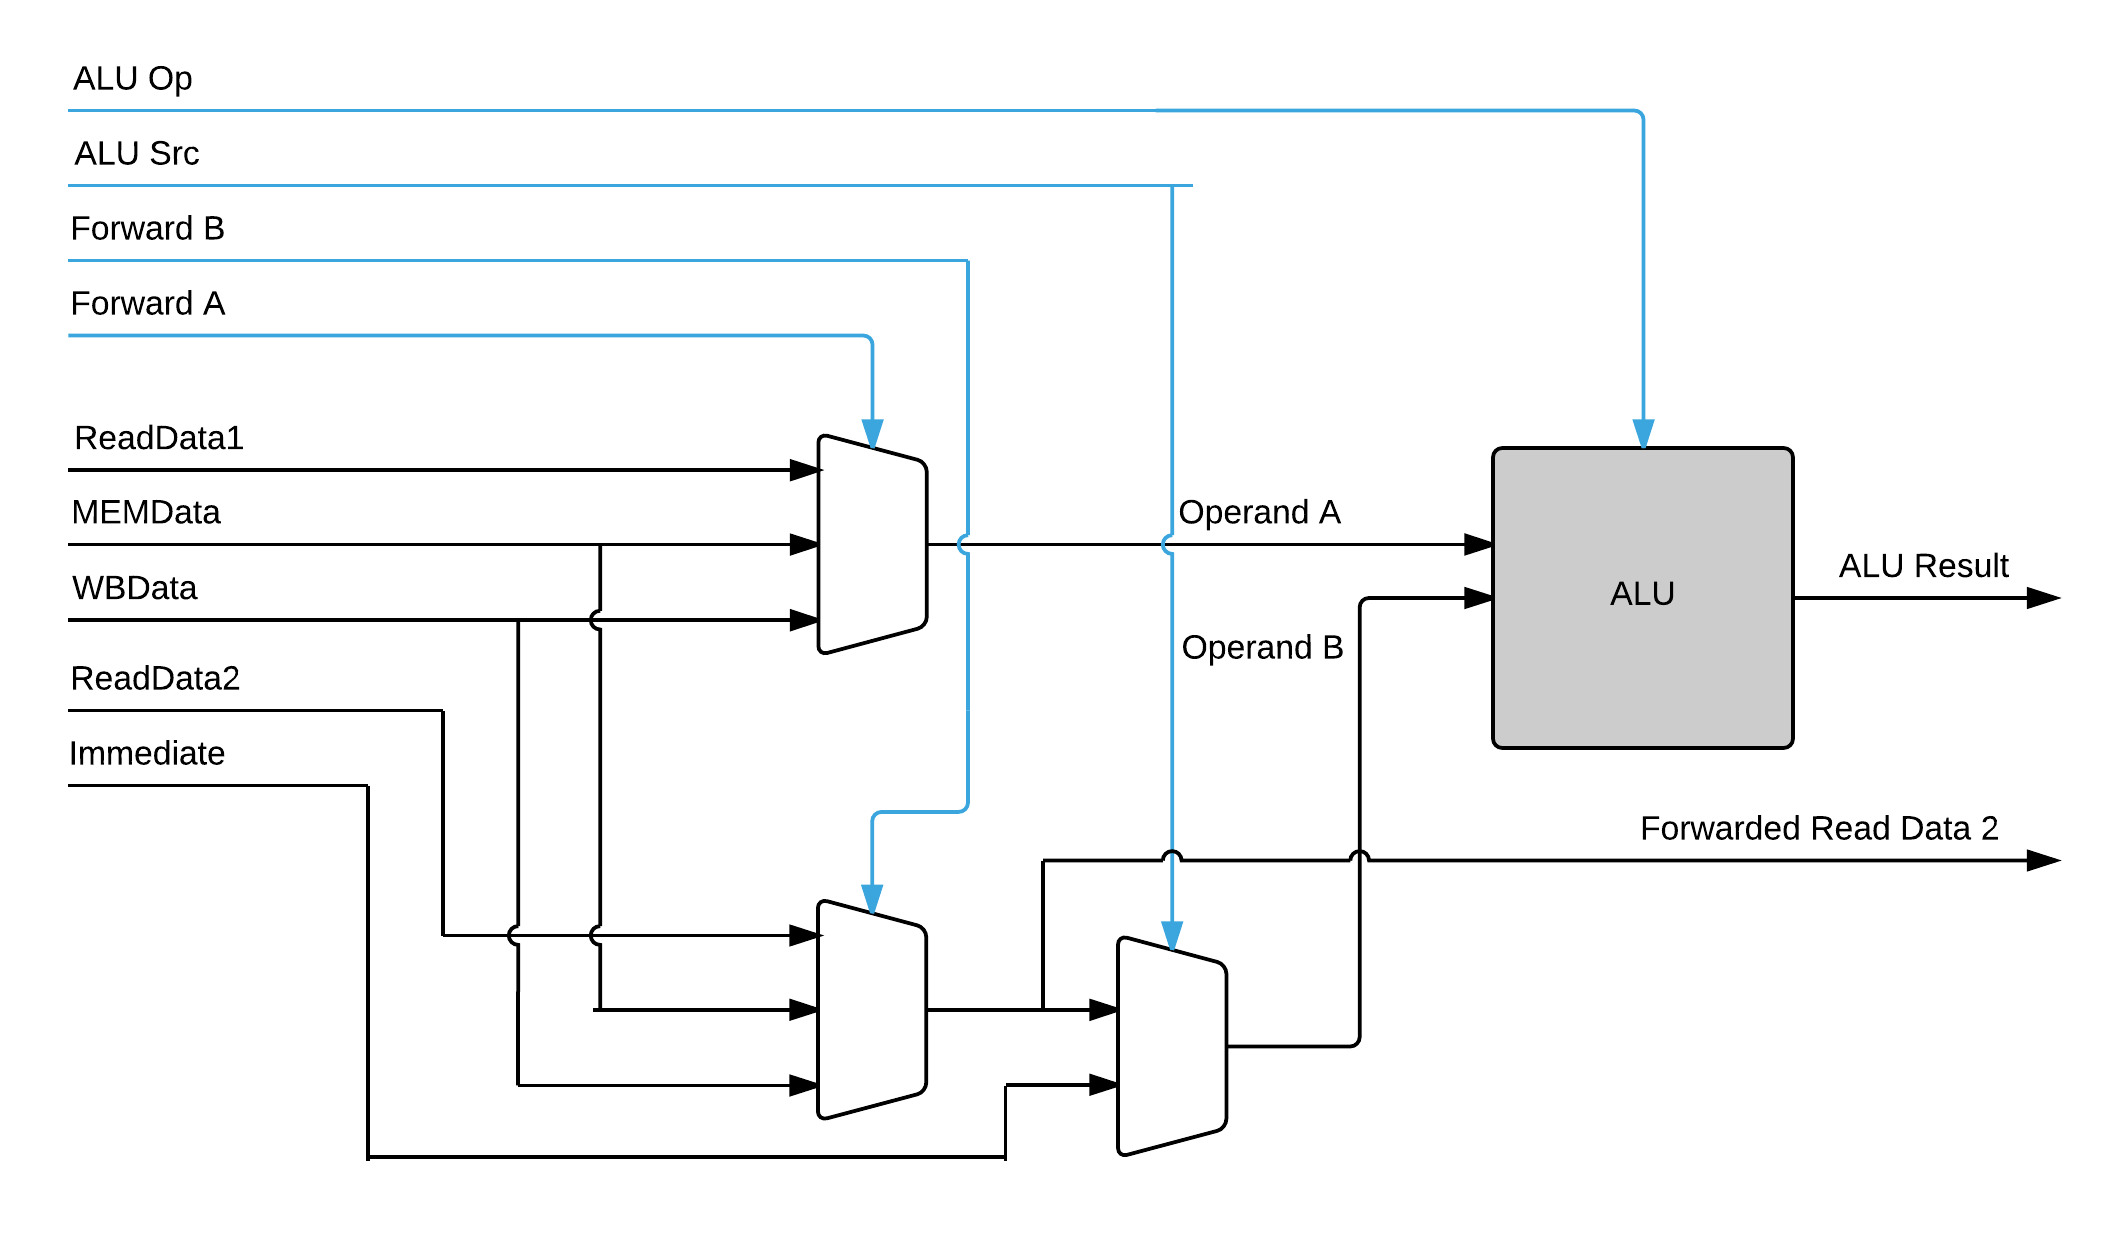
\includegraphics[width=\linewidth]{img/ALU.png}
    \caption{RTL Schematic of the ALU}
    \label{fig:ALU}
\end{figure}

\subsection{Registers}

\subsection{Branch}

\subsection{Forwarder}
\label{section:Forwarder}
The forwarder, as described in the ALU section, overrides registe reads when more recent data is available further down the pipeline.
The task of the forwarder is to check, for both operands, whether either of the operands reads data from the destination register of an operation further down the pipeline.
First the source register for both of the source register (or, in case of i-format instructions, the source register) of the operation in the execute stage is compared with the destination register of the operation currently in mem stage. 
If either operand in execute stage reads from the destination register of the operation currently at the mem stage, the forwarder forwards this data in place of the register data.
If an operand is not found as the result in the mem stage, the forwarder checks the WB stage.
As with the mem stage, if a source register at the execute stage is similar to a destination register in the wb stage it is selected as operand source by the forwarder. 
This ensures that in the case where the same destination register is used both in the mem stage and the wb stage the most recent one will be chosen.
Note that the forwarder checks forwarding for each source register independently, allowing an instruction to use any combination of reg, mem and wb as its source registers.
In our design this ensures that all dependencies are taken care of except for the case when an instruction is dependant on a result from a load operation which takes an extra cycle before being available at the MEM stage.
In addition to forwarding data for the execute stage the forwarder has one more task:
In the case where an instruction in the ID stage uses data from the destination register of the operation in the WB stage the job of the forwarder is to select the write data signal instead of the register read signal.
This is nescessary because the instruction relies on data that cannot be forwarded once it reaches the execute stage, but is not updated in the register file before the instruction that needs it has already read the old value from the register file.

\subsection{Hazard detection}

\subsection{Pipeline registers}

